\section{Software design}
\textcolor{red}{some general info}

\subsection{Peripherals} %please think about the appropriate name!
The description of our modular architecture, the work principles of the separate modules and basically "how we control the peripherals" such as motors, leds, timers, etc. Logic comes a bit later in here.
Also all info on DMA and pin remapping and our pretty mapping table are also welcomed here I think

\subsubsection*{Timer 1}
\textcolor{red}{
Short description on how we worked out the time
}

\subsubsection*{Pulse Width Modulation (PWM)}

\begin{figure}[htb]
    \centering
    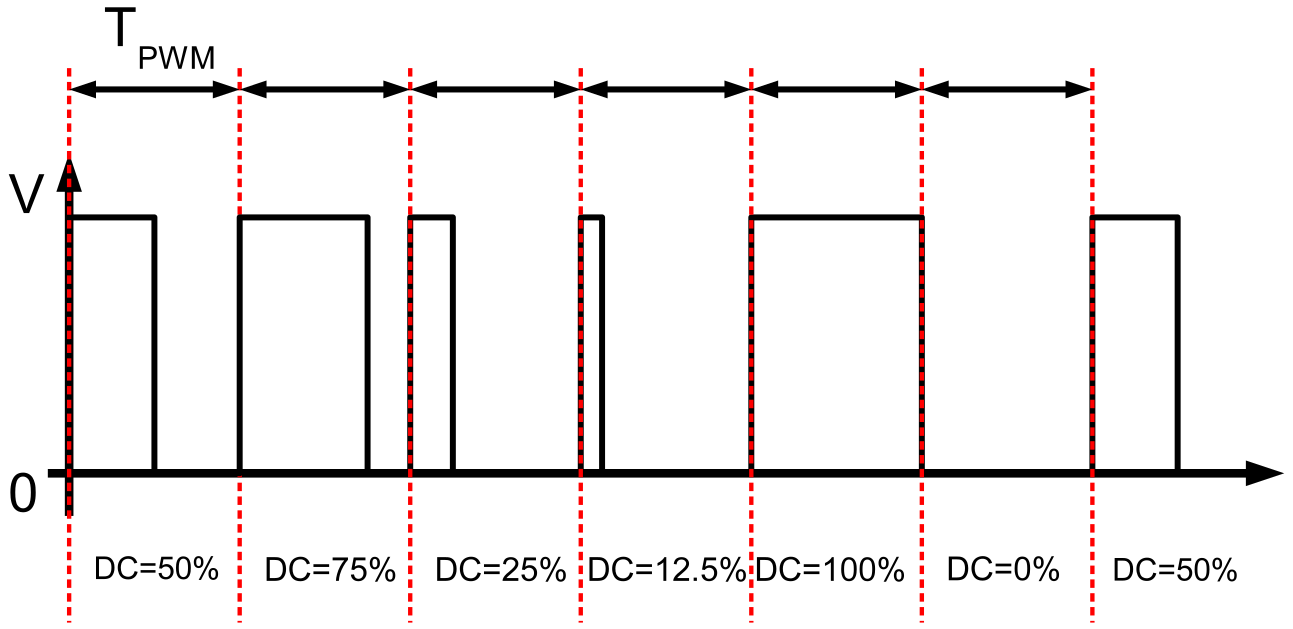
\includegraphics[width=0.6\textwidth]{figures/software/pwm_demo.png}
    \caption {Principle of PWM \cite{alex}}
    \label{fig:pwm_demo}
\end{figure}

Pulse Width Modulation allows us to control the amount of energy supplied to an actuator. In this case we use the PWM signal to drive our motors and control their speed. Using different pulse widths, we can supply different amount of power to our motors. \cite{alex}


As seen in figure \ref{fig:pwm_demo}, we have a fixed PWM period $T_{PWM}$. We can now vary the so called duty cycle $DC$ by changing the time the PWM output is switched on ($T_{DC}$).
\begin{equation}
    DC = \frac{T_{DC}}{T_{PWM}}
\end{equation}
For our PWM unit, we mainly have to choose the parameters:
\begin{enumerate}
    \item PWM period
    \item PWM duty cycle
\end{enumerate}


Depending on our PWM period, we get different amount of ripple in our resulting signal. More on this can be found in \cite[Chapter~5.1]{alex}. In figure \ref{fig:pwm_choice} is an example of possible choices for the PWM period register ($PTPER$) and the PWM duty cycle register ($PDC$)

\begin{figure}[htb]
    \centering
    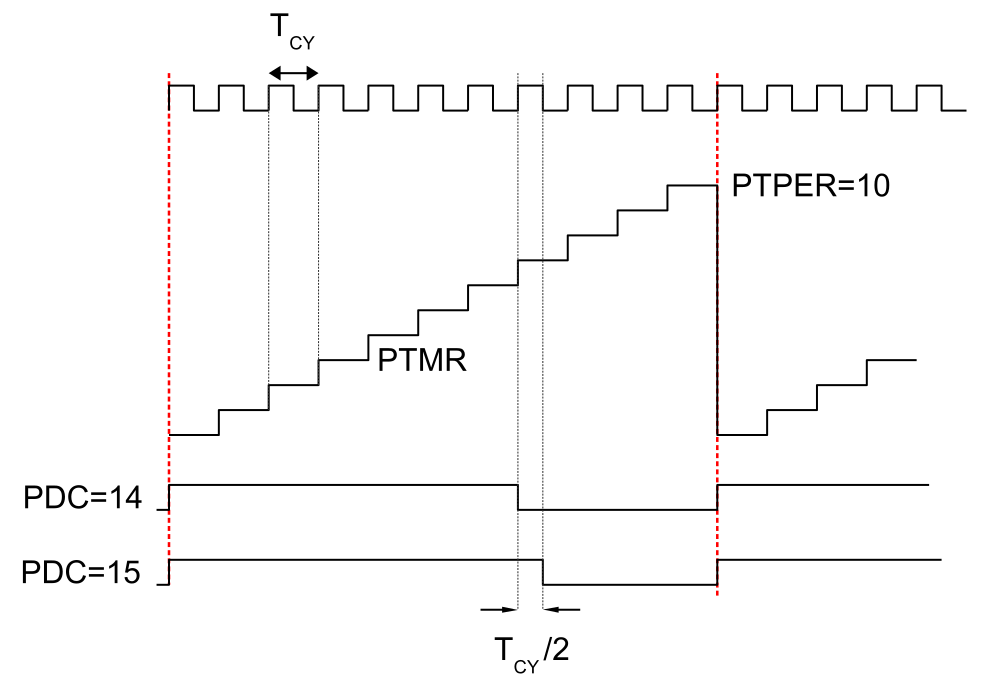
\includegraphics[width=0.6\textwidth]{figures/software/pwm_choice.png}
    \caption {Example: Resolution of PWM duty cycle \cite{alex}}
    \label{fig:pwm_choice}
\end{figure}

For our motors, we have the following parameters:
\begin{itemize}
    \item \textbf{fixed}: $T_{CY} = 25 ns$
    \item timer prescaler $PTCKPS = 0b00$ (option 1:1)
    \item PWM period register $P1TPER = 2000 - 1$
    \item PWM duty cycle $PDC \in [0, 2*(P1TPER + 1)]$
\end{itemize}
$T_{PWM} = ( PTPER + 1 ) * T_{CY} = 2000 * 25ns = 50000 ns$


$f_{PWM} = \frac{1}{T_{PWM}} = 0.25 * 10^{5} Hz$

With the current values, we can now set different duty cycles for our motors by choosing valid values for the $PDC$ register.


\subsubsection*{Quadrature Encoder Inferface(QEI)}
To measure the position and velocity of our motors, we are provided with a \textit{quadrature encoder}. The principle of a quadrature encoder is depicted in figure \ref{fig:qei_demo}. 

\begin{figure}[htb]
    \centering
    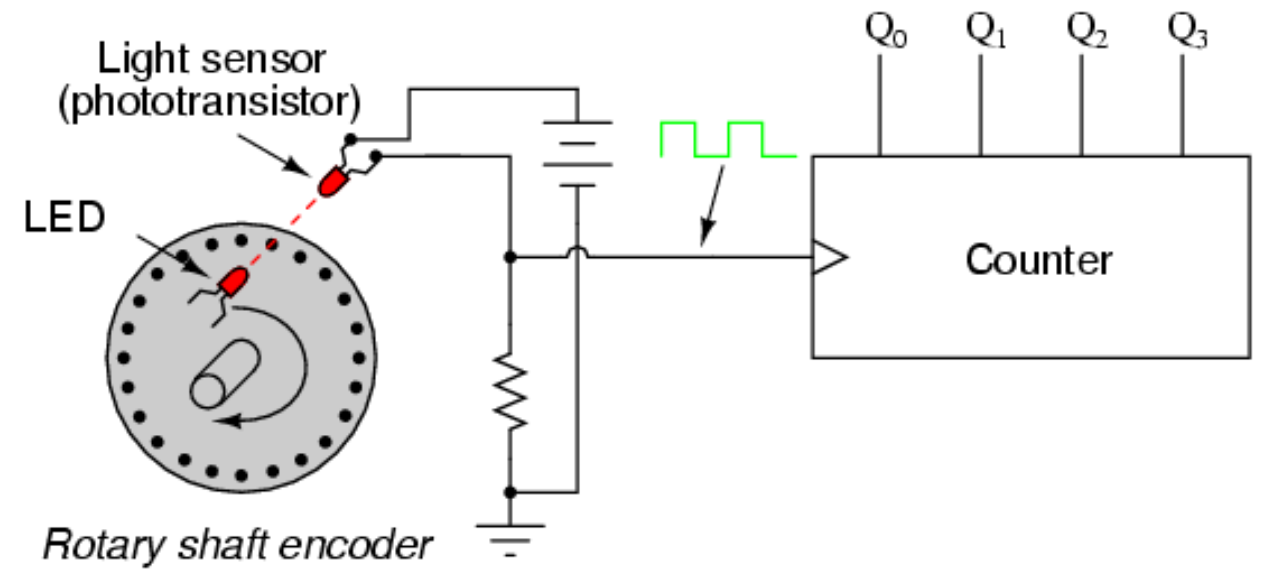
\includegraphics[width=0.6\textwidth]{figures/software/qei_demo.png}
    \caption {Principle of a rotary shaft encoder \cite{alex}}
    \label{fig:qei_demo}
\end{figure}

Whenever the wheel is rotated, light emitted from the LED will hit the light sensor (phototransistor) if there is a hole between them. Light sensor and emitter are separated by the wheel seen in \ref{fig:qei_demo}.
The time passed between the phototransistor turning on after registering light and turning off again after the light disappears behind the wheel will determine the velocity of our motor.


\subsubsection*{Analogue-to-Digital Conversion(ADC)}

\subsubsection*{Direct Memory Access (DMA) - does this belong here?}

\subsubsection*{Universal Asynchronous Receiver Transmitter (UART)}
Our dsPIC33FJ64MC804 has a Universal Asynchronous Receiver Transmitter (UART)  module for serial port communication.
The UART can communicate with peripheral devices. 
In our case, we use it to commmunicate with an outside computer to send commands or read out values. This was especially useful to find fitting parameters for our gains in the controller logic (chapter).

\begin{figure}[htb]
    \centering
    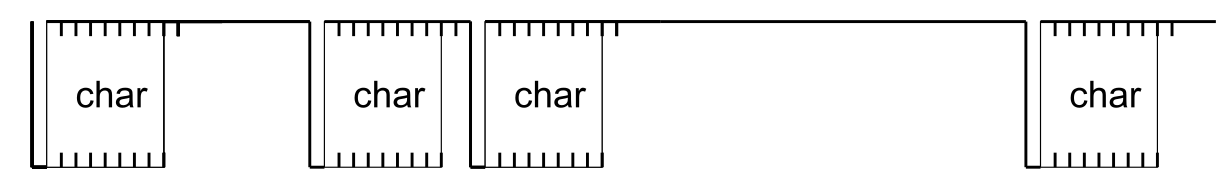
\includegraphics[width=0.6\textwidth]{figures/software/uart_demo.png}
    \caption {String transmission of 8 bit characters with one start bit and one stop bit (no parity) \cite{alex}}
    \label{fig:uart_demo}
\end{figure}

Figure \ref{fig:uart_demo} shows the transmission of a string consisting of three characters. 
The dsPIC33FJ64MC804 allows us to specify the properties of our transmission. The most important settings:
\begin{itemize}
    \item Baud rate: 57.6 kbit/s
    \item Data Selection Bits: 8
    \item Parity bit: 0
    \item Stop bit: 1
\end{itemize}

In order to send out messages, we require another module. We therefore connect our microcontroller to the \textbf{HC-05 Bluetooth Module} (figure \ref{fig:hc_05} so that we can send messages to that module which again transfers those messages via bluetooth to our computer where we read out the values.

\begin{figure}[htb]
    \centering
    \begin{minipage}{.5\textwidth}
          \centering
            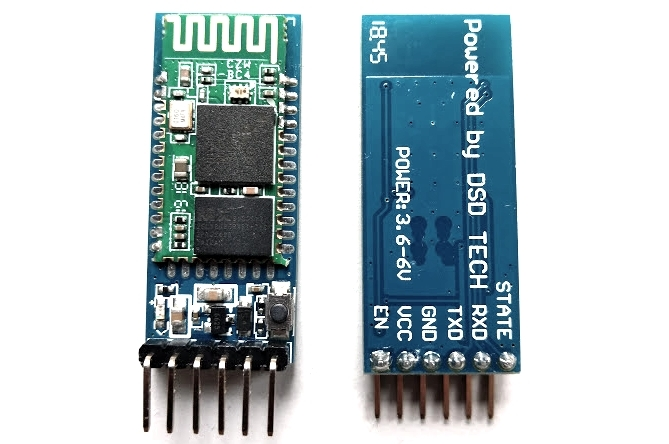
\includegraphics[width=.9\linewidth]{figures/software/uart_hc05.jpg}
              \caption{HC-05 Bluetooth Module}
                \label{fig:hc_05}
    \end{minipage}%
    \begin{minipage}{.5\textwidth}
          \centering
            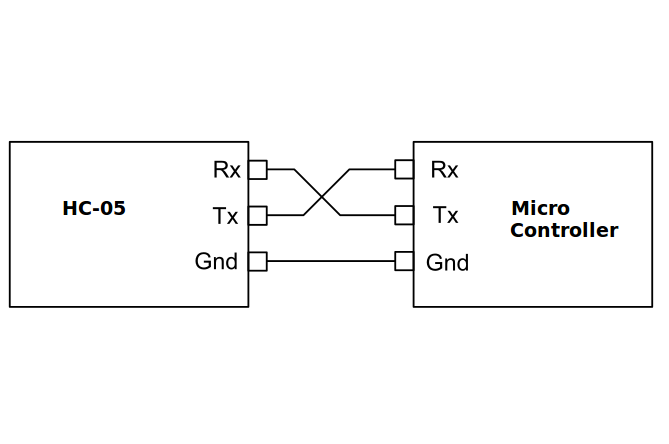
\includegraphics[width=.9\linewidth]{figures/software/uart_plug.png}
              \caption{Connecting the HC-05 module to our microcontroller}
                \label{fig:wire_3}
    \end{minipage}
\end{figure}

The 3-wire UART as seen in figure \ref{fig:wire_3} shows our configuration for a full-duplex communication. The Bluetooth module sends out the message it gets on the reception line (Rx) and sends back messages to the microcontroller through its transmission line (Tx). To receive the message from our microcontroller, we need to connect our computer to the HC-05 module via bluetooth.

It is important to configure the baud rate of the HC-05 module in advance, such that it matches our microcontroller's baud rate. Also, in order to read out values, the baud rate on the PC we are reading from, must also match (in this case 57.6 kbit/s)

\subsection{Pin Mapping}
\textcolor{red}{
maybe a diagram of which peripheral maps to which pin
}


\subsection{Controller Design and Approach}

\textcolor{red}{
Here goes the whole logic of the mouse movement control (how should it behave when is faced with the wall or on contrary - with the gap in the labyrinth). PID controller design and the logic behind it.
}

\subsubsection{Proportional-Integral-Derivative Controller (PID)}

\subsubsection{State Machine}



